\documentclass[openany]{book}
\usepackage{lmodern}
\usepackage{amssymb,amsmath}
\usepackage{ifxetex,ifluatex}
\usepackage{fixltx2e} % provides \textsubscript
\ifnum 0\ifxetex 1\fi\ifluatex 1\fi=0 % if pdftex
  \usepackage[T1]{fontenc}
  \usepackage[utf8]{inputenc}
\else % if luatex or xelatex
  \ifxetex
    \usepackage{mathspec}
  \else
    \usepackage{fontspec}
  \fi
  \defaultfontfeatures{Ligatures=TeX,Scale=MatchLowercase}
\fi
% use upquote if available, for straight quotes in verbatim environments
\IfFileExists{upquote.sty}{\usepackage{upquote}}{}
% use microtype if available
\IfFileExists{microtype.sty}{%
\usepackage{microtype}
\UseMicrotypeSet[protrusion]{basicmath} % disable protrusion for tt fonts
}{}
\usepackage[margin=1in]{geometry}
\usepackage{hyperref}
\hypersetup{unicode=true,
            pdftitle={DATA 624: Project 1 - Part B},
            pdfauthor={Sang Yoon (Andy) Hwang \& Vinicio Haro},
            pdfborder={0 0 0},
            breaklinks=true}
\urlstyle{same}  % don't use monospace font for urls
\usepackage{natbib}
\bibliographystyle{plainnat}
\usepackage{color}
\usepackage{fancyvrb}
\newcommand{\VerbBar}{|}
\newcommand{\VERB}{\Verb[commandchars=\\\{\}]}
\DefineVerbatimEnvironment{Highlighting}{Verbatim}{commandchars=\\\{\}}
% Add ',fontsize=\small' for more characters per line
\usepackage{framed}
\definecolor{shadecolor}{RGB}{248,248,248}
\newenvironment{Shaded}{\begin{snugshade}}{\end{snugshade}}
\newcommand{\KeywordTok}[1]{\textcolor[rgb]{0.13,0.29,0.53}{\textbf{#1}}}
\newcommand{\DataTypeTok}[1]{\textcolor[rgb]{0.13,0.29,0.53}{#1}}
\newcommand{\DecValTok}[1]{\textcolor[rgb]{0.00,0.00,0.81}{#1}}
\newcommand{\BaseNTok}[1]{\textcolor[rgb]{0.00,0.00,0.81}{#1}}
\newcommand{\FloatTok}[1]{\textcolor[rgb]{0.00,0.00,0.81}{#1}}
\newcommand{\ConstantTok}[1]{\textcolor[rgb]{0.00,0.00,0.00}{#1}}
\newcommand{\CharTok}[1]{\textcolor[rgb]{0.31,0.60,0.02}{#1}}
\newcommand{\SpecialCharTok}[1]{\textcolor[rgb]{0.00,0.00,0.00}{#1}}
\newcommand{\StringTok}[1]{\textcolor[rgb]{0.31,0.60,0.02}{#1}}
\newcommand{\VerbatimStringTok}[1]{\textcolor[rgb]{0.31,0.60,0.02}{#1}}
\newcommand{\SpecialStringTok}[1]{\textcolor[rgb]{0.31,0.60,0.02}{#1}}
\newcommand{\ImportTok}[1]{#1}
\newcommand{\CommentTok}[1]{\textcolor[rgb]{0.56,0.35,0.01}{\textit{#1}}}
\newcommand{\DocumentationTok}[1]{\textcolor[rgb]{0.56,0.35,0.01}{\textbf{\textit{#1}}}}
\newcommand{\AnnotationTok}[1]{\textcolor[rgb]{0.56,0.35,0.01}{\textbf{\textit{#1}}}}
\newcommand{\CommentVarTok}[1]{\textcolor[rgb]{0.56,0.35,0.01}{\textbf{\textit{#1}}}}
\newcommand{\OtherTok}[1]{\textcolor[rgb]{0.56,0.35,0.01}{#1}}
\newcommand{\FunctionTok}[1]{\textcolor[rgb]{0.00,0.00,0.00}{#1}}
\newcommand{\VariableTok}[1]{\textcolor[rgb]{0.00,0.00,0.00}{#1}}
\newcommand{\ControlFlowTok}[1]{\textcolor[rgb]{0.13,0.29,0.53}{\textbf{#1}}}
\newcommand{\OperatorTok}[1]{\textcolor[rgb]{0.81,0.36,0.00}{\textbf{#1}}}
\newcommand{\BuiltInTok}[1]{#1}
\newcommand{\ExtensionTok}[1]{#1}
\newcommand{\PreprocessorTok}[1]{\textcolor[rgb]{0.56,0.35,0.01}{\textit{#1}}}
\newcommand{\AttributeTok}[1]{\textcolor[rgb]{0.77,0.63,0.00}{#1}}
\newcommand{\RegionMarkerTok}[1]{#1}
\newcommand{\InformationTok}[1]{\textcolor[rgb]{0.56,0.35,0.01}{\textbf{\textit{#1}}}}
\newcommand{\WarningTok}[1]{\textcolor[rgb]{0.56,0.35,0.01}{\textbf{\textit{#1}}}}
\newcommand{\AlertTok}[1]{\textcolor[rgb]{0.94,0.16,0.16}{#1}}
\newcommand{\ErrorTok}[1]{\textcolor[rgb]{0.64,0.00,0.00}{\textbf{#1}}}
\newcommand{\NormalTok}[1]{#1}
\usepackage{graphicx,grffile}
\makeatletter
\def\maxwidth{\ifdim\Gin@nat@width>\linewidth\linewidth\else\Gin@nat@width\fi}
\def\maxheight{\ifdim\Gin@nat@height>\textheight\textheight\else\Gin@nat@height\fi}
\makeatother
% Scale images if necessary, so that they will not overflow the page
% margins by default, and it is still possible to overwrite the defaults
% using explicit options in \includegraphics[width, height, ...]{}
\setkeys{Gin}{width=\maxwidth,height=\maxheight,keepaspectratio}
\IfFileExists{parskip.sty}{%
\usepackage{parskip}
}{% else
\setlength{\parindent}{0pt}
\setlength{\parskip}{6pt plus 2pt minus 1pt}
}
\setlength{\emergencystretch}{3em}  % prevent overfull lines
\providecommand{\tightlist}{%
  \setlength{\itemsep}{0pt}\setlength{\parskip}{0pt}}
\setcounter{secnumdepth}{5}

%%% Use protect on footnotes to avoid problems with footnotes in titles
\let\rmarkdownfootnote\footnote%
\def\footnote{\protect\rmarkdownfootnote}

%%% Change title format to be more compact
\usepackage{titling}

% Create subtitle command for use in maketitle
\newcommand{\subtitle}[1]{
  \posttitle{
    \begin{center}\large#1\end{center}
    }
}

\setlength{\droptitle}{-2em}

  \title{DATA 624: Project 1 - Part B}
    \pretitle{\vspace{\droptitle}\centering\huge}
  \posttitle{\par}
    \author{Sang Yoon (Andy) Hwang \& Vinicio Haro}
    \preauthor{\centering\large\emph}
  \postauthor{\par}
      \predate{\centering\large\emph}
  \postdate{\par}
    \date{October 22, 2019}

\usepackage{booktabs}
\usepackage[table]{xcolor}

% set plain style for page numbers
\pagestyle{plain}
\raggedbottom

% change font
\usepackage{fontspec}
\setmainfont{Arial}

% remove "chapter" from chapter title
\usepackage{titlesec}
\titleformat{\chapter}
  {\normalfont\LARGE\bfseries}{\thechapter}{1em}{}
\titlespacing*{\chapter}{0pt}{3.5ex plus 1ex minus .2ex}{2.3ex plus .2ex}

% create color block quotes
\usepackage{tcolorbox}
\newtcolorbox{myquote}{colback=orange!05!white, colframe=black!75!black}
\renewenvironment{quote}{\begin{myquote}}{\end{myquote}}

% wrap text
\usepackage{geometry}[textwidth=6in]

% kable 
\usepackage{tabu}
\usepackage{float}
\usepackage{booktabs}
\usepackage{longtable}
\usepackage{array}
\usepackage{multirow}
\usepackage{wrapfig}
\usepackage{float}
\usepackage{colortbl}
\usepackage{pdflscape}
\usepackage{tabu}
\usepackage{threeparttable}
\usepackage{threeparttablex}
\usepackage[normalem]{ulem}
\usepackage{makecell}
\usepackage{xcolor}

\begin{document}
\maketitle

{
\setcounter{tocdepth}{1}
\tableofcontents
}
\chapter*{Part B: Forecasting Power}\label{part-b}
\addcontentsline{toc}{chapter}{Part B: Forecasting Power}

\begin{quote}
\textbf{Instructions:} Part B consists of a simple dataset of
residential power usage for January 1998 until December 2013. Your
assignment is to model these data and a monthly forecast for 2014. The
data is given in a single file. The variable `KWH' is power consumption
in Kilowatt hours, the rest is straight forward. Add these to your
existing files above - clearly labeled.
\end{quote}

\section*{Data Exploration and Processing}\label{b-exploration}
\addcontentsline{toc}{section}{Data Exploration and Processing}

Explore data. Process as needed.

\begin{Shaded}
\begin{Highlighting}[]
\KeywordTok{library}\NormalTok{(tidyverse)}
\KeywordTok{library}\NormalTok{(scales)}
\KeywordTok{library}\NormalTok{(readxl)}
\KeywordTok{library}\NormalTok{(forecast)}
\KeywordTok{library}\NormalTok{(lubridate)}
\KeywordTok{library}\NormalTok{(fpp2)}
\KeywordTok{library}\NormalTok{(ggplot2)}
\KeywordTok{library}\NormalTok{(forecast)}
\KeywordTok{library}\NormalTok{(tseries)}
\KeywordTok{library}\NormalTok{(imputeTS)}
\KeywordTok{library}\NormalTok{(tsoutliers)}
\CommentTok{#install.packages('tsoutliers')}
\end{Highlighting}
\end{Shaded}

\begin{Shaded}
\begin{Highlighting}[]
\CommentTok{#power_data <- read_excel("data/ResidentialCustomerForecastLoad-624.xlsx") }
\KeywordTok{library}\NormalTok{ (readr)}

\NormalTok{power=}\StringTok{"https://raw.githubusercontent.com/vindication09/DATA-624/master/ResidentialCustomerForecastLoad-624.csv"}

\NormalTok{partb_data<-}\KeywordTok{read_csv}\NormalTok{(}\KeywordTok{url}\NormalTok{(power))}

\KeywordTok{head}\NormalTok{(partb_data)}
\end{Highlighting}
\end{Shaded}

\begin{verbatim}
FALSE # A tibble: 6 x 3
FALSE   CaseSequence `YYYY-MMM`     KWH
FALSE          <dbl> <chr>        <dbl>
FALSE 1          733 1998-Jan   6862583
FALSE 2          734 1998-Feb   5838198
FALSE 3          735 1998-Mar   5420658
FALSE 4          736 1998-Apr   5010364
FALSE 5          737 1998-May   4665377
FALSE 6          738 1998-Jun   6467147
\end{verbatim}

Transformed data into time-series with freq - 12.

\begin{Shaded}
\begin{Highlighting}[]
\NormalTok{ts_data <-}\StringTok{ }\KeywordTok{ts}\NormalTok{(partb_data}\OperatorTok{$}\NormalTok{KWH, }\DataTypeTok{frequency =} \DecValTok{12}\NormalTok{, }\DataTypeTok{start =} \KeywordTok{c}\NormalTok{(}\DecValTok{1998}\NormalTok{,}\DecValTok{1}\NormalTok{))}
\end{Highlighting}
\end{Shaded}

Missing value check

\begin{Shaded}
\begin{Highlighting}[]
\KeywordTok{sum}\NormalTok{(}\KeywordTok{is.na}\NormalTok{(ts_data))}
\end{Highlighting}
\end{Shaded}

\begin{verbatim}
FALSE [1] 1
\end{verbatim}

Impute Missing Data using TSImpute

\begin{Shaded}
\begin{Highlighting}[]
\NormalTok{ts_data<-}\KeywordTok{na.interpolation}\NormalTok{(ts_data)}
\end{Highlighting}
\end{Shaded}

Review the cycle of the time series to get an idea of the positions
within the cycle.

\begin{Shaded}
\begin{Highlighting}[]
\KeywordTok{cycle}\NormalTok{(ts_data)}
\end{Highlighting}
\end{Shaded}

\begin{verbatim}
FALSE      Jan Feb Mar Apr May Jun Jul Aug Sep Oct Nov Dec
FALSE 1998   1   2   3   4   5   6   7   8   9  10  11  12
FALSE 1999   1   2   3   4   5   6   7   8   9  10  11  12
FALSE 2000   1   2   3   4   5   6   7   8   9  10  11  12
FALSE 2001   1   2   3   4   5   6   7   8   9  10  11  12
FALSE 2002   1   2   3   4   5   6   7   8   9  10  11  12
FALSE 2003   1   2   3   4   5   6   7   8   9  10  11  12
FALSE 2004   1   2   3   4   5   6   7   8   9  10  11  12
FALSE 2005   1   2   3   4   5   6   7   8   9  10  11  12
FALSE 2006   1   2   3   4   5   6   7   8   9  10  11  12
FALSE 2007   1   2   3   4   5   6   7   8   9  10  11  12
FALSE 2008   1   2   3   4   5   6   7   8   9  10  11  12
FALSE 2009   1   2   3   4   5   6   7   8   9  10  11  12
FALSE 2010   1   2   3   4   5   6   7   8   9  10  11  12
FALSE 2011   1   2   3   4   5   6   7   8   9  10  11  12
FALSE 2012   1   2   3   4   5   6   7   8   9  10  11  12
FALSE 2013   1   2   3   4   5   6   7   8   9  10  11  12
\end{verbatim}

Summary Statistics

\begin{Shaded}
\begin{Highlighting}[]
\KeywordTok{summary}\NormalTok{(ts_data)}
\end{Highlighting}
\end{Shaded}

\begin{verbatim}
FALSE     Min.  1st Qu.   Median     Mean  3rd Qu.     Max. 
FALSE   770523  5434539  6314472  6502824  7608792 10655730
\end{verbatim}

\begin{Shaded}
\begin{Highlighting}[]
\CommentTok{#disable scientific notation (ONLY RUN ONCE)}
\KeywordTok{options}\NormalTok{(}\DataTypeTok{scipen =} \DecValTok{99999}\NormalTok{)}

\KeywordTok{autoplot}\NormalTok{(ts_data) }\OperatorTok{+}
\KeywordTok{labs}\NormalTok{(}\DataTypeTok{title =} \StringTok{"Monthly Residential Power Usage"}\NormalTok{, }\DataTypeTok{subtitle =} \StringTok{"01/98 - 12/13"}\NormalTok{)}\OperatorTok{+}
\KeywordTok{theme_classic}\NormalTok{();}
\end{Highlighting}
\end{Shaded}

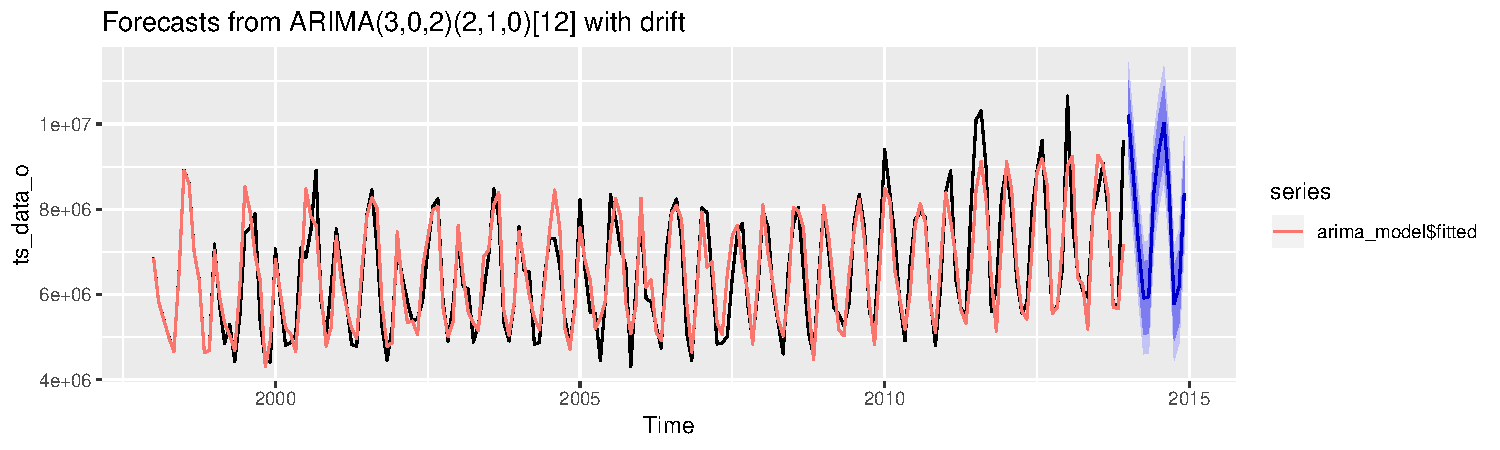
\includegraphics{Part-B-AS_files/figure-latex/unnamed-chunk-8-1.pdf}

\begin{Shaded}
\begin{Highlighting}[]
\KeywordTok{ggseasonplot}\NormalTok{(ts_data);}
\end{Highlighting}
\end{Shaded}

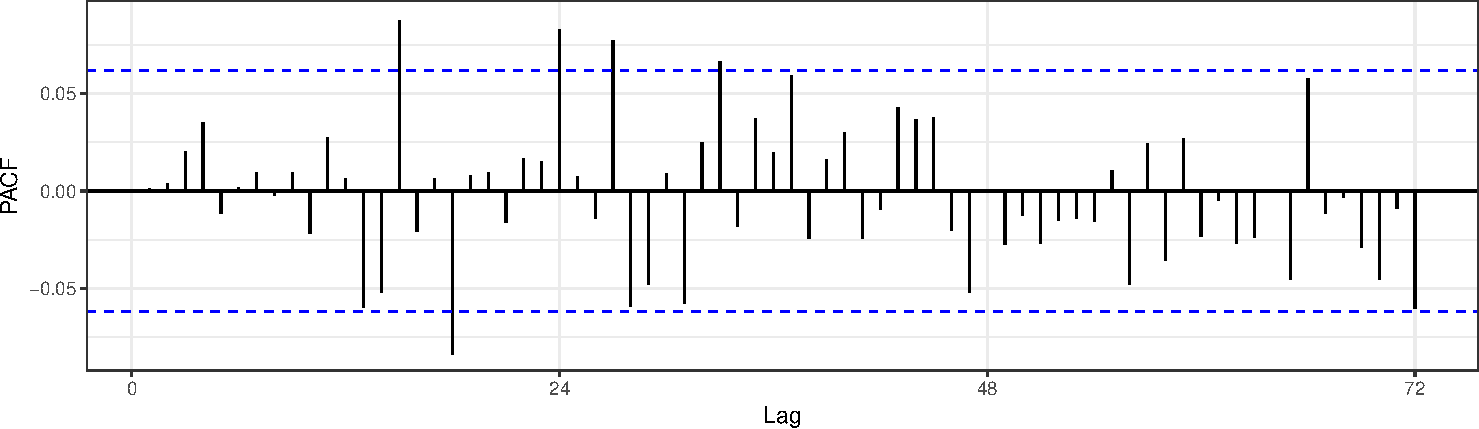
\includegraphics{Part-B-AS_files/figure-latex/unnamed-chunk-8-2.pdf}

\begin{Shaded}
\begin{Highlighting}[]
\KeywordTok{boxplot}\NormalTok{(ts_data}\OperatorTok{~}\KeywordTok{cycle}\NormalTok{(ts_data),}\DataTypeTok{xlab=}\StringTok{"Month"}\NormalTok{, }\DataTypeTok{ylab =} \StringTok{"Monthly Residential Power Usage"}\NormalTok{);}
\end{Highlighting}
\end{Shaded}

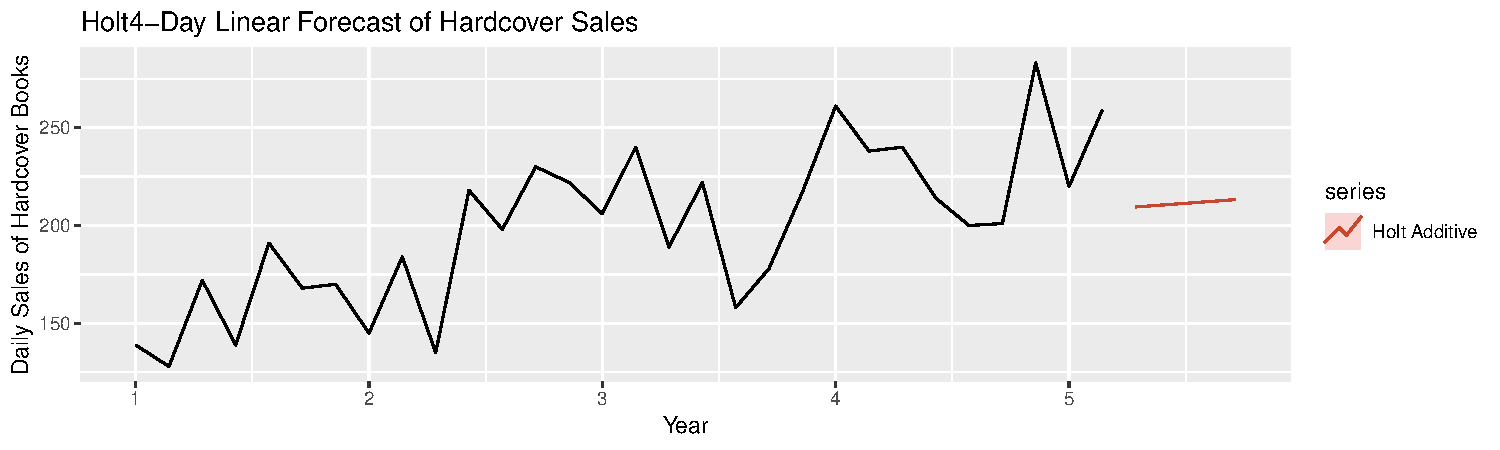
\includegraphics{Part-B-AS_files/figure-latex/unnamed-chunk-8-3.pdf}

\begin{Shaded}
\begin{Highlighting}[]
\KeywordTok{ggsubseriesplot}\NormalTok{(ts_data);}
\end{Highlighting}
\end{Shaded}

\includegraphics{Part-B-AS_files/figure-latex/unnamed-chunk-8-4.pdf}

\begin{Shaded}
\begin{Highlighting}[]
\KeywordTok{stl}\NormalTok{(ts_data, }\DataTypeTok{s.window =} \StringTok{'periodic'}\NormalTok{) }\OperatorTok\StringTok{ }\KeywordTok{autoplot}\NormalTok{();}
\end{Highlighting}
\end{Shaded}

\includegraphics{Part-B-AS_files/figure-latex/unnamed-chunk-8-5.pdf}

\begin{Shaded}
\begin{Highlighting}[]
\KeywordTok{ggAcf}\NormalTok{(ts_data);}
\end{Highlighting}
\end{Shaded}

\includegraphics{Part-B-AS_files/figure-latex/unnamed-chunk-8-6.pdf}

\begin{Shaded}
\begin{Highlighting}[]
\KeywordTok{tsoutliers}\NormalTok{(ts_data, }\DataTypeTok{iterate =} \DecValTok{2}\NormalTok{, }\DataTypeTok{lambda =} \StringTok{"auto"}\NormalTok{)}
\end{Highlighting}
\end{Shaded}

\begin{verbatim}
FALSE $index
FALSE [1] 151
FALSE 
FALSE $replacements
FALSE [1] 7757226
\end{verbatim}

Our initial plots reveal annual seasonality within this time series. The
box plot/seasonality plot actually reveals where power consumption
fluctuations occur within each of the cycke positions. We can speculate
that this could be due to there being no major Holidays that require
power draining decor plus we assume minimal AC usage during the cold
months.

We see power consumption increase between the months of June and August.
This must be tied to AC usage during the warmer months of a year and
finally power usage dips from September to Novemeber with a small spike
in December. We speculate that thisis due to transitioning out of
summer. The spike in December could be connected to the usage or Holiday
lights being kept on.

Within the overall TS plot, we see a dip in July 2010. This could be due
to a power outtage during a hot summer month. This can certainly be
considered to be an outlier within this TS. Using TSOutliers, we can
actually identify the index where our outliers may be. TSoutliers also
replaces the outlier using Box-Cox. If set lambda=auto, then TSoutliers
will automatically perform Box-Cox transformation.

The ACF plot shows that autocorrelations are well outside the
significant space indicating white noise.

\section*{Data Model}\label{b-model}
\addcontentsline{toc}{section}{Data Model}

\subsection{Model \#1: ARIMA}\label{model-1-arima}

\begin{Shaded}
\begin{Highlighting}[]
\NormalTok{arima_model <-}\StringTok{ }\KeywordTok{auto.arima}\NormalTok{(ts_data)}

\NormalTok{arima_model <-}\StringTok{ }\KeywordTok{forecast}\NormalTok{(arima_model, }\DataTypeTok{h=}\DecValTok{12}\NormalTok{)}

\KeywordTok{autoplot}\NormalTok{(arima_model) }\OperatorTok{+}\StringTok{ }\KeywordTok{autolayer}\NormalTok{(}\KeywordTok{fitted}\NormalTok{(arima_model))}
\end{Highlighting}
\end{Shaded}

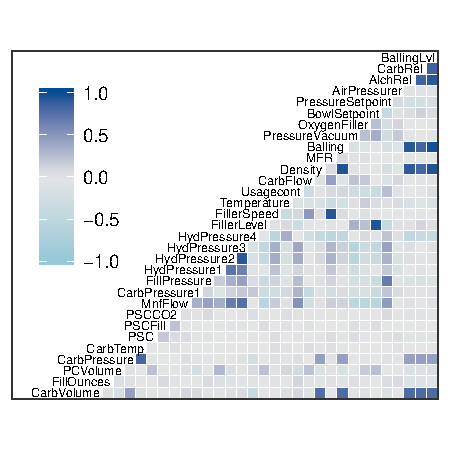
\includegraphics{Part-B-AS_files/figure-latex/unnamed-chunk-9-1.pdf}

\begin{Shaded}
\begin{Highlighting}[]
\KeywordTok{checkresiduals}\NormalTok{(arima_model)}
\end{Highlighting}
\end{Shaded}

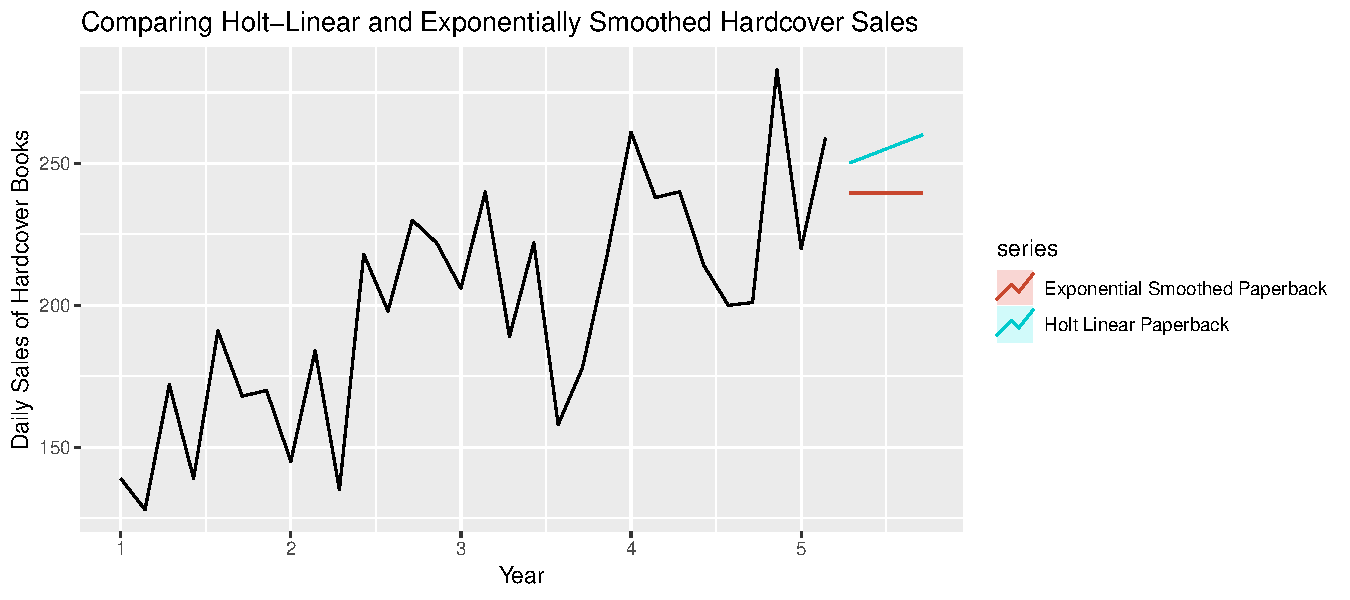
\includegraphics{Part-B-AS_files/figure-latex/unnamed-chunk-9-2.pdf}

\begin{verbatim}
FALSE 
FALSE   Ljung-Box test
FALSE 
FALSE data:  Residuals from ARIMA(0,0,1)(1,1,1)[12] with drift
FALSE Q* = 14.209, df = 20, p-value = 0.8197
FALSE 
FALSE Model df: 4.   Total lags used: 24
\end{verbatim}

\subsection{Model \#2: STL (no-demped) -
ANN}\label{model-2-stl-no-demped---ann}

\begin{Shaded}
\begin{Highlighting}[]
\CommentTok{#stlf - etsmodel estimation --- A,N,N is chosen.}
\NormalTok{stl_ndemp <-}\StringTok{ }\KeywordTok{stlf}\NormalTok{(ts_data, }\DataTypeTok{damped=}\OtherTok{FALSE}\NormalTok{, }\DataTypeTok{s.window =} \StringTok{"periodic"}\NormalTok{, }\DataTypeTok{robust=}\OtherTok{TRUE}\NormalTok{, }\DataTypeTok{h =} \DecValTok{12}\NormalTok{)}

\CommentTok{# forecast plot}
\KeywordTok{autoplot}\NormalTok{(stl_ndemp) }\OperatorTok{+}\StringTok{ }\KeywordTok{autolayer}\NormalTok{(}\KeywordTok{fitted}\NormalTok{(stl_ndemp))}
\end{Highlighting}
\end{Shaded}

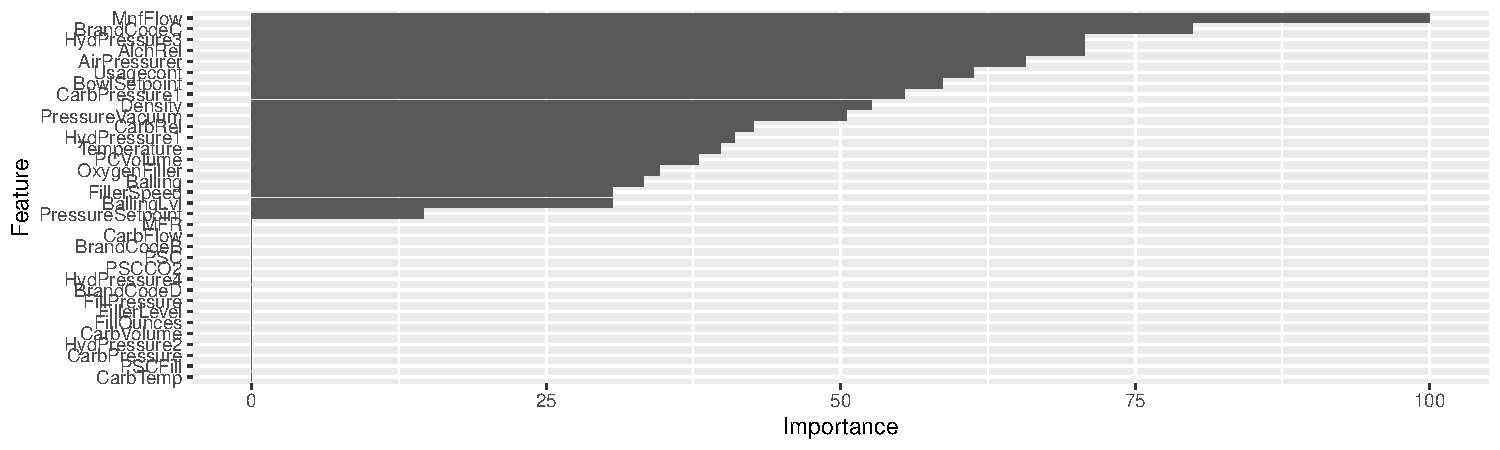
\includegraphics{Part-B-AS_files/figure-latex/unnamed-chunk-10-1.pdf}

\begin{Shaded}
\begin{Highlighting}[]
\KeywordTok{checkresiduals}\NormalTok{(stl_ndemp)}
\end{Highlighting}
\end{Shaded}

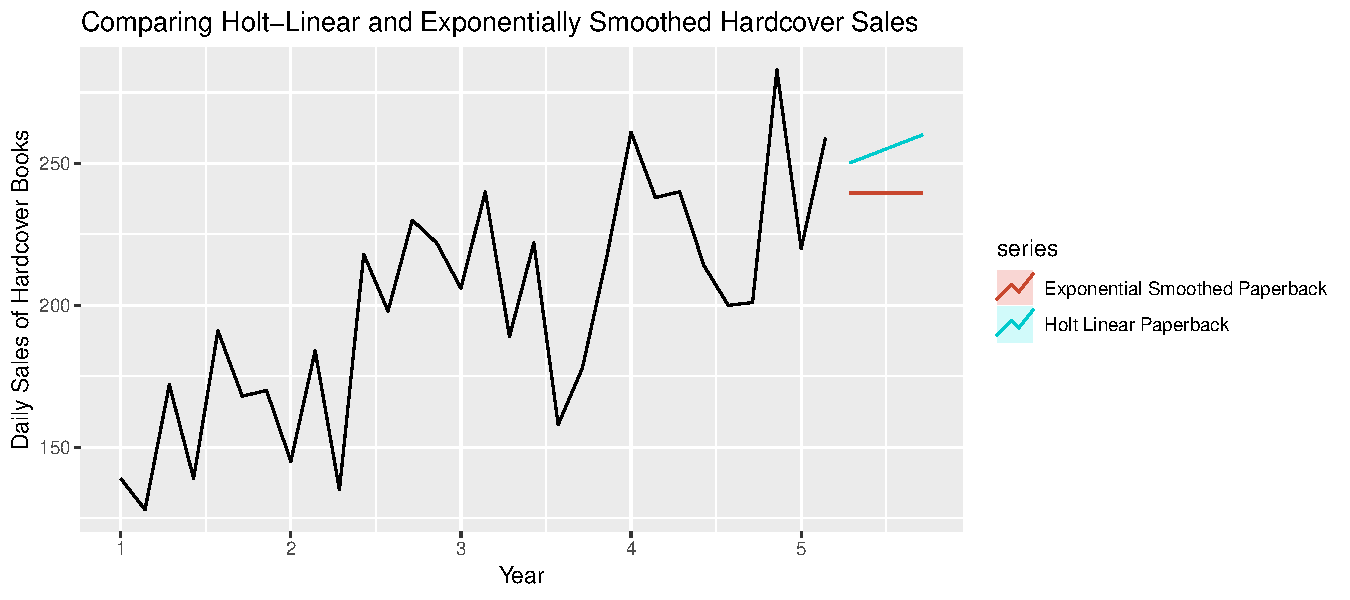
\includegraphics{Part-B-AS_files/figure-latex/unnamed-chunk-10-2.pdf}

\begin{verbatim}
FALSE 
FALSE   Ljung-Box test
FALSE 
FALSE data:  Residuals from STL +  ETS(A,N,N)
FALSE Q* = 27.948, df = 22, p-value = 0.1774
FALSE 
FALSE Model df: 2.   Total lags used: 24
\end{verbatim}

\chapter{Model \#2-2: STL (demped) -
AAdN}\label{model-2-2-stl-demped---aadn}

\begin{Shaded}
\begin{Highlighting}[]
\CommentTok{#stlf - etsmodel estimation --- M, Ad, N is chosen.}
\NormalTok{stl_demp <-}\StringTok{ }\KeywordTok{stlf}\NormalTok{(ts_data, }\DataTypeTok{damped=}\OtherTok{TRUE}\NormalTok{, }\DataTypeTok{s.window =} \StringTok{"periodic"}\NormalTok{, }\DataTypeTok{robust=}\OtherTok{TRUE}\NormalTok{, }\DataTypeTok{h =} \DecValTok{12}\NormalTok{)}

\CommentTok{# forecast plot}
\KeywordTok{autoplot}\NormalTok{(stl_demp) }\OperatorTok{+}\StringTok{ }\KeywordTok{autolayer}\NormalTok{(}\KeywordTok{fitted}\NormalTok{(stl_demp))}
\end{Highlighting}
\end{Shaded}

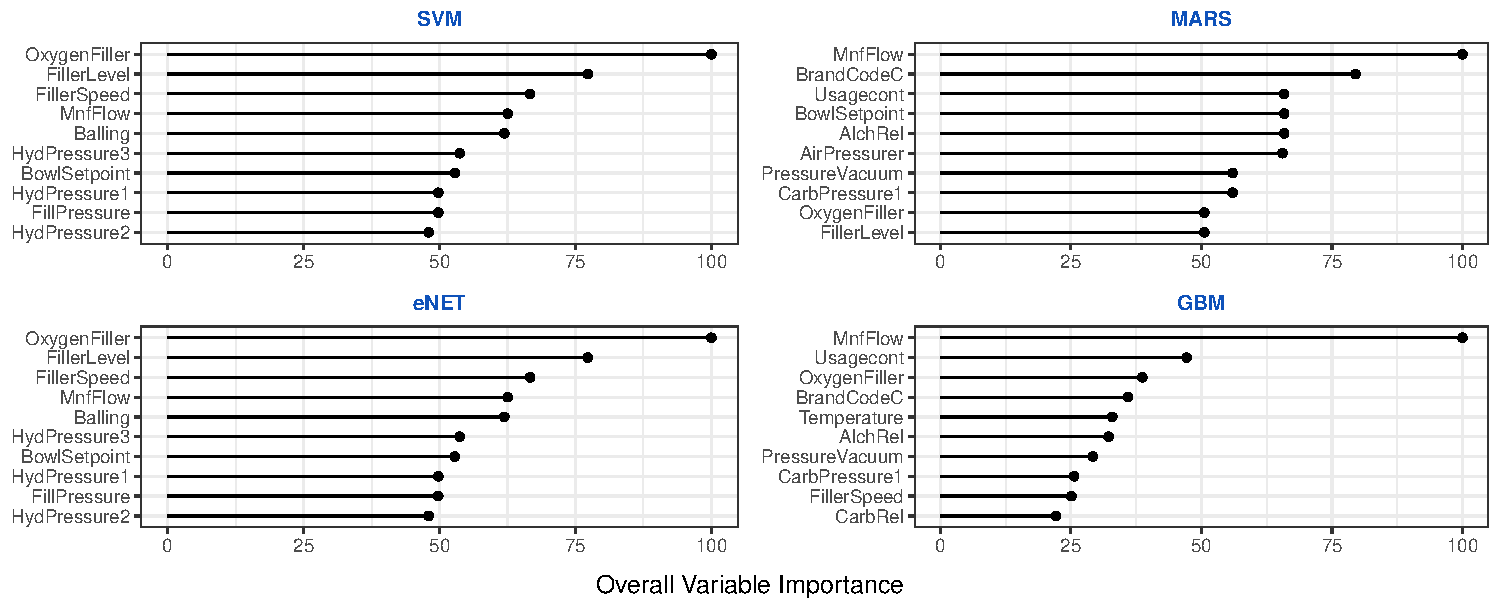
\includegraphics{Part-B-AS_files/figure-latex/unnamed-chunk-11-1.pdf}

\begin{Shaded}
\begin{Highlighting}[]
\KeywordTok{checkresiduals}\NormalTok{(stl_demp)}
\end{Highlighting}
\end{Shaded}

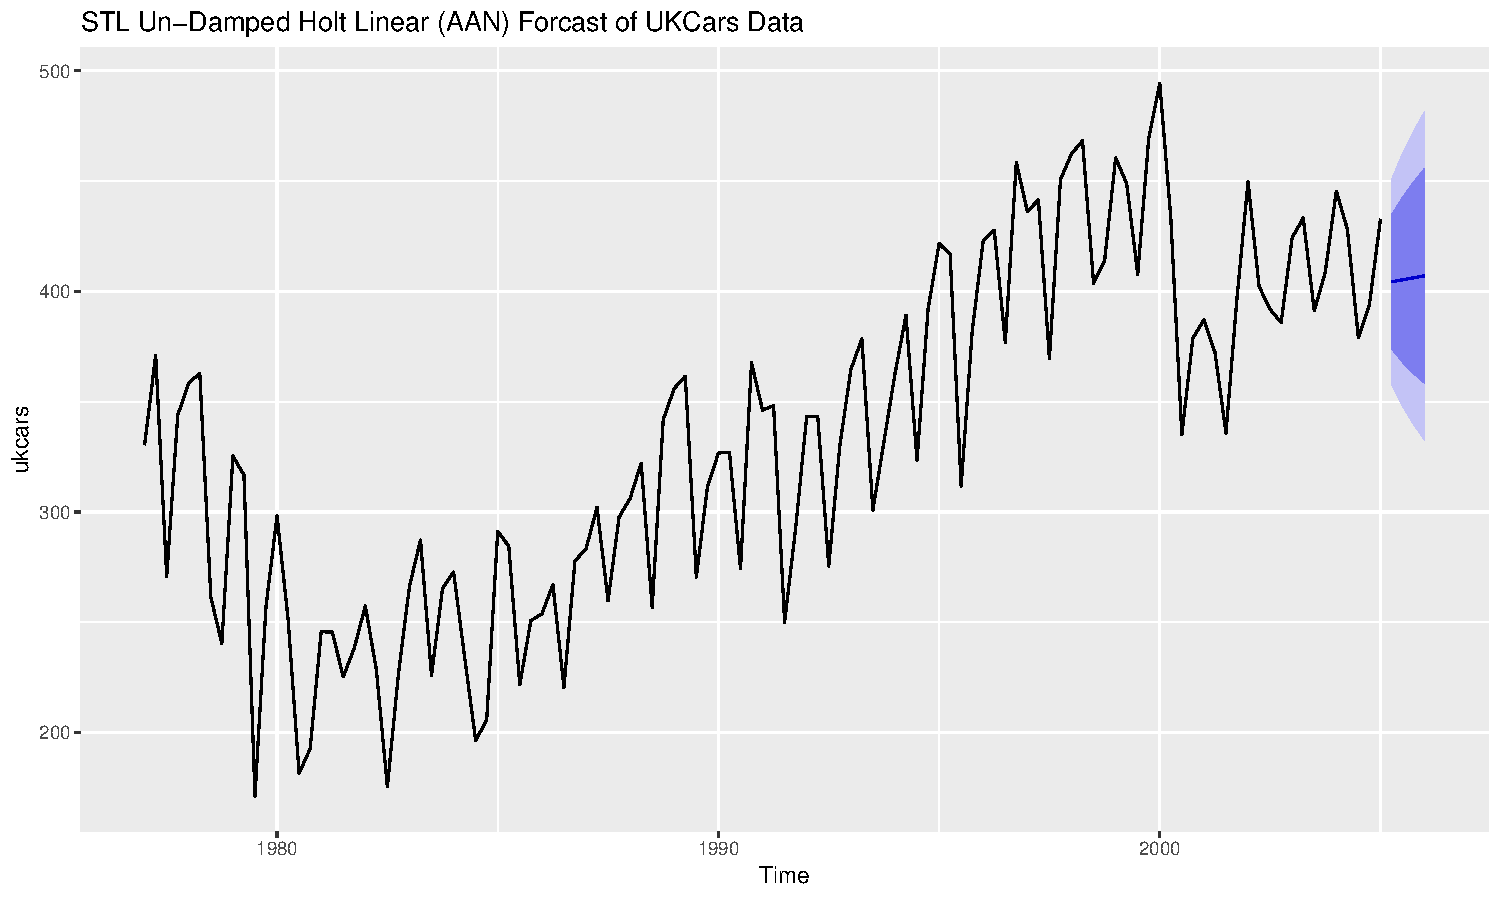
\includegraphics{Part-B-AS_files/figure-latex/unnamed-chunk-11-2.pdf}

\begin{verbatim}
FALSE 
FALSE   Ljung-Box test
FALSE 
FALSE data:  Residuals from STL +  ETS(A,Ad,N)
FALSE Q* = 26.06, df = 19, p-value = 0.1285
FALSE 
FALSE Model df: 5.   Total lags used: 24
\end{verbatim}

\chapter{Model \#3: ets - MNM}\label{model-3-ets---mnm}

\begin{Shaded}
\begin{Highlighting}[]
\CommentTok{# ETS models - MNM}
\NormalTok{ets_model <-}\StringTok{ }\KeywordTok{ets}\NormalTok{(ts_data)}

\CommentTok{# forecast plot}
\KeywordTok{autoplot}\NormalTok{(}\KeywordTok{forecast}\NormalTok{(ets_model, }\DataTypeTok{h=}\DecValTok{12}\NormalTok{)) }\OperatorTok{+}\StringTok{ }\KeywordTok{autolayer}\NormalTok{(}\KeywordTok{fitted}\NormalTok{(ets_model))}
\end{Highlighting}
\end{Shaded}

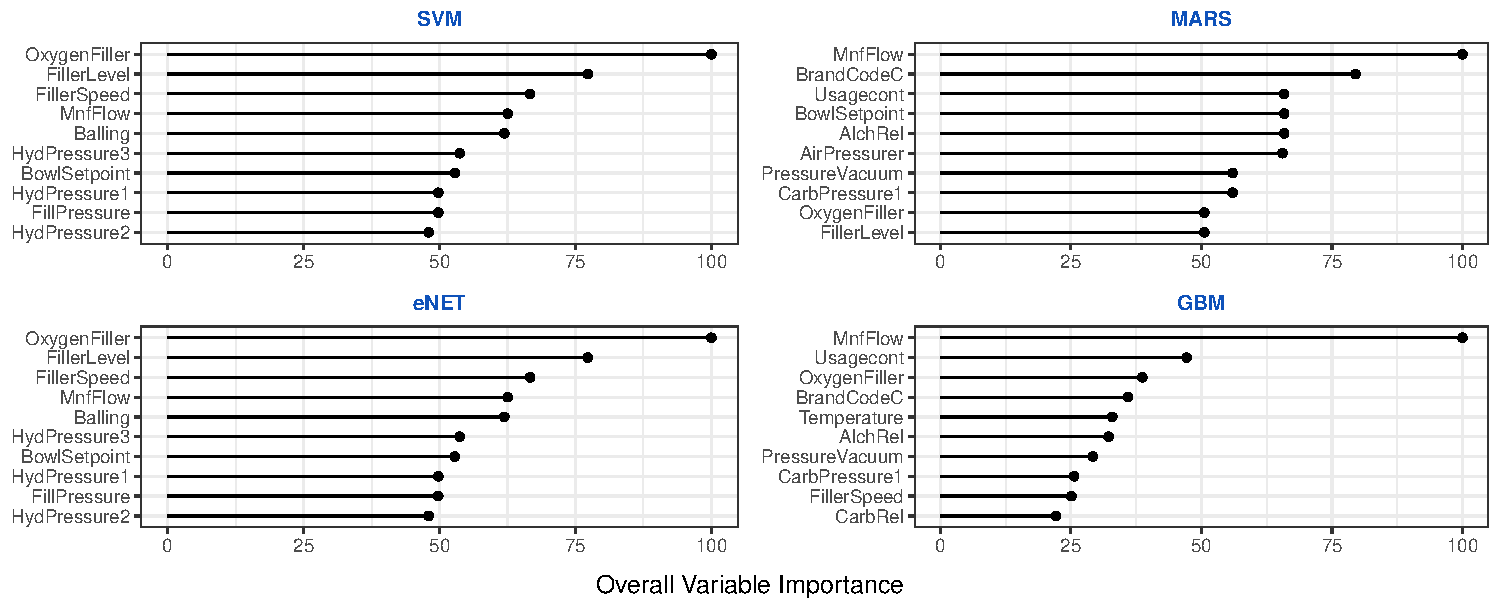
\includegraphics{Part-B-AS_files/figure-latex/unnamed-chunk-12-1.pdf}

\begin{Shaded}
\begin{Highlighting}[]
\KeywordTok{checkresiduals}\NormalTok{(ets_model)}
\end{Highlighting}
\end{Shaded}

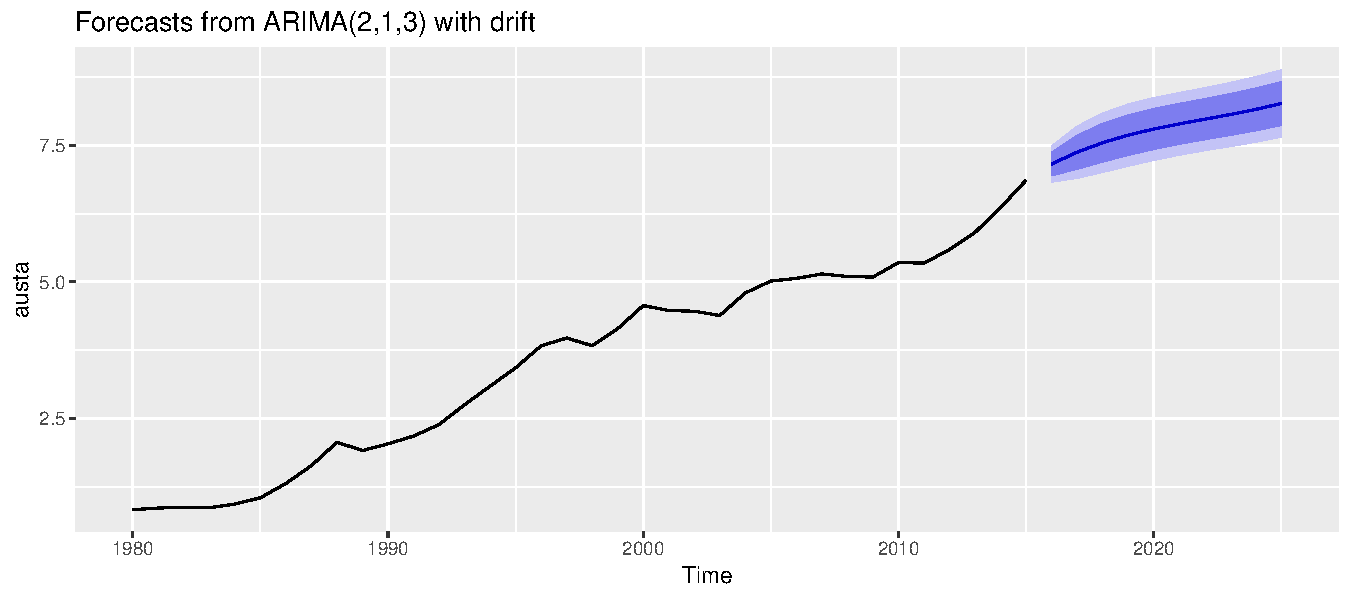
\includegraphics{Part-B-AS_files/figure-latex/unnamed-chunk-12-2.pdf}

\begin{verbatim}
FALSE 
FALSE   Ljung-Box test
FALSE 
FALSE data:  Residuals from ETS(M,N,M)
FALSE Q* = 28.615, df = 10, p-value = 0.001438
FALSE 
FALSE Model df: 14.   Total lags used: 24
\end{verbatim}

Accuracy of Models

\begin{Shaded}
\begin{Highlighting}[]
\KeywordTok{accuracy}\NormalTok{(arima_model);}
\end{Highlighting}
\end{Shaded}

\begin{verbatim}
FALSE                     ME     RMSE      MAE       MPE   MAPE      MASE
FALSE Training set -25089.69 827254.2 493308.5 -5.511184 11.685 0.7080556
FALSE                    ACF1
FALSE Training set 0.01283694
\end{verbatim}

\begin{Shaded}
\begin{Highlighting}[]
\KeywordTok{accuracy}\NormalTok{(stl_ndemp);}
\end{Highlighting}
\end{Shaded}

\begin{verbatim}
FALSE                    ME     RMSE      MAE      MPE     MAPE      MASE
FALSE Training set 70019.52 841778.6 510068.7 -4.24069 12.00083 0.7321119
FALSE                   ACF1
FALSE Training set 0.2096288
\end{verbatim}

\begin{Shaded}
\begin{Highlighting}[]
\KeywordTok{accuracy}\NormalTok{(stl_demp);}
\end{Highlighting}
\end{Shaded}

\begin{verbatim}
FALSE                    ME     RMSE      MAE       MPE     MAPE      MASE
FALSE Training set 55479.88 841315.3 509435.8 -4.493116 12.03609 0.7312034
FALSE                   ACF1
FALSE Training set 0.2087849
\end{verbatim}

\begin{Shaded}
\begin{Highlighting}[]
\KeywordTok{accuracy}\NormalTok{(ets_model)}
\end{Highlighting}
\end{Shaded}

\begin{verbatim}
FALSE                    ME   RMSE      MAE      MPE     MAPE      MASE
FALSE Training set 61009.73 835107 503972.9 -4.39013 12.04006 0.7233624
FALSE                   ACF1
FALSE Training set 0.1698584
\end{verbatim}

Out of the models we built,we can make some preliminary observations.
The residuals for each of our models does not have a major deviance from
normality, however Model \#1: ARIMA residuals do not have an extended
number of bins distorting the normality proximity.

The ACF plots show autocorrelations for each of our 4 models. Model \#1:
ARIMA has less autocorrelation than the other three models. Model 1 is
well within the 95\% limits indicated by the dotted blue lines.

If we examine the Ljung-Box test results for our models, the only model
with a pvalue \textless{} 0.05 is Model \#3: ets - MNM. This implies
that the residuals are not independent.

\section*{Forecast}\label{b-forecast}
\addcontentsline{toc}{section}{Forecast}

We will impliment a cross validation method of testing for h=12. The
process randomly chooses 12 points to measure and generate the RMSE.By
definition, a lower RMSE is attributed with a better fit.

\chapter{Model \#1: ARIMA}\label{model-1-arima-1}

\begin{Shaded}
\begin{Highlighting}[]
\NormalTok{arima_cv <-}\StringTok{ }\ControlFlowTok{function}\NormalTok{(x, h)\{}\KeywordTok{forecast}\NormalTok{(}\KeywordTok{Arima}\NormalTok{(ts_data, }\DataTypeTok{order =} \KeywordTok{c}\NormalTok{(}\DecValTok{0}\NormalTok{, }\DecValTok{0}\NormalTok{, }\DecValTok{1}\NormalTok{), }\DataTypeTok{seasonal =} \KeywordTok{c}\NormalTok{(}\DecValTok{1}\NormalTok{, }\DecValTok{1}\NormalTok{, }\DecValTok{1}\NormalTok{),  }\DataTypeTok{include.drift =} \OtherTok{TRUE}\NormalTok{), }\DataTypeTok{h=}\NormalTok{h)\}}
\NormalTok{e <-}\StringTok{ }\KeywordTok{tsCV}\NormalTok{(ts_data, arima_cv, }\DataTypeTok{h=}\DecValTok{12}\NormalTok{)}

\KeywordTok{sqrt}\NormalTok{(}\KeywordTok{mean}\NormalTok{(e}\OperatorTok{^}\DecValTok{2}\NormalTok{, }\DataTypeTok{na.rm=}\OtherTok{TRUE}\NormalTok{))}
\end{Highlighting}
\end{Shaded}

\begin{verbatim}
FALSE [1] 2135370
\end{verbatim}

\chapter{Model \#2: STL (no-demped) -
ANN}\label{model-2-stl-no-demped---ann-1}

\begin{Shaded}
\begin{Highlighting}[]
\NormalTok{e <-}\StringTok{ }\KeywordTok{tsCV}\NormalTok{(ts_data, stlf, }\DataTypeTok{damped=}\OtherTok{FALSE}\NormalTok{, }\DataTypeTok{s.window =} \StringTok{"periodic"}\NormalTok{, }\DataTypeTok{robust=}\OtherTok{TRUE}\NormalTok{, }\DataTypeTok{h=}\DecValTok{12}\NormalTok{)}

\KeywordTok{sqrt}\NormalTok{(}\KeywordTok{mean}\NormalTok{(e}\OperatorTok{^}\DecValTok{2}\NormalTok{, }\DataTypeTok{na.rm=}\OtherTok{TRUE}\NormalTok{))}
\end{Highlighting}
\end{Shaded}

\begin{verbatim}
FALSE [1] 1014297
\end{verbatim}

\chapter{Model \#2-2: STL (demped) -
AAdN}\label{model-2-2-stl-demped---aadn-1}

\begin{Shaded}
\begin{Highlighting}[]
\NormalTok{e <-}\StringTok{ }\KeywordTok{tsCV}\NormalTok{(ts_data, stlf, }\DataTypeTok{damped=}\OtherTok{TRUE}\NormalTok{, }\DataTypeTok{s.window =} \StringTok{"periodic"}\NormalTok{, }\DataTypeTok{robust=}\OtherTok{TRUE}\NormalTok{, }\DataTypeTok{h=}\DecValTok{12}\NormalTok{)}

\KeywordTok{sqrt}\NormalTok{(}\KeywordTok{mean}\NormalTok{(e}\OperatorTok{^}\DecValTok{2}\NormalTok{, }\DataTypeTok{na.rm=}\OtherTok{TRUE}\NormalTok{))}
\end{Highlighting}
\end{Shaded}

\begin{verbatim}
FALSE [1] 1018495
\end{verbatim}

Using Time series cross-validation, we compute RMSE on testset (h=12).
We will pick the model with the lowest RMSE on testset as our final
model. ARIMA is the worst predictor in terms of RMSE on test set (the
highest RMSE) which shows that the model is seriously overfitted - low
bias but very high variance. Surprisingly, STL (no-demped) - ANN, which
was the worst predictor in terms of RMSE on training set, has the lowest
RMSE on test set among all models. Since this is yearly forecast, tsCV(h
= 12) would make sense.

\section*{Discussion}\label{b-discussion}
\addcontentsline{toc}{section}{Discussion}

Given that 4 models we created did not vary much in terms of RMSE on
training, while STL - ANN has significantly lower RMSE on test set than
ARIMA, we will choose STL - ANN as our final model.

We found that ARIMA is the worst predictor and STL - AAN is the best
model as RMSE on test set is the lowest, contradicting to its' RMSE on
train set. It comes down to the discussion of bias-variance trade off;
overfitted model cannot generalize the outcome of predictions on unseen
data well.


\end{document}
